% 2020 江苏卷 第18题 题图：单圆锥曲线与少量直线
% 椭圆 x^2/4 + y^2/3 = 1，F1(-1,0), F2(1,0)
% A(1,3/2) 在第一象限且 AF2 垂直 F1F2，直线 AF1 与椭圆另交于 B
\usetikzlibrary{arrows.meta}
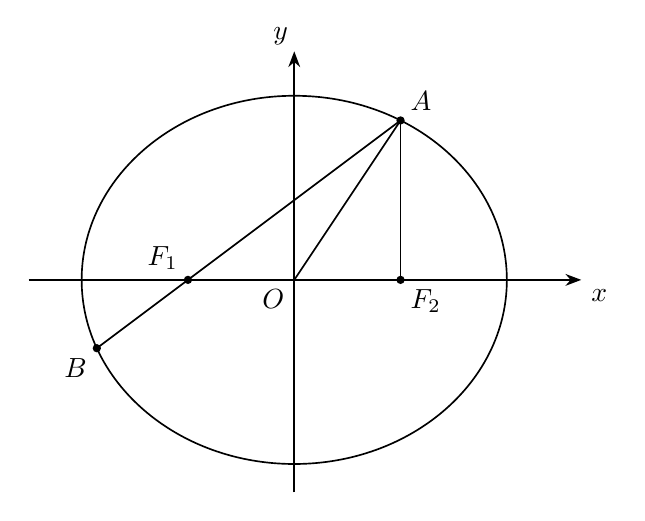
\begin{tikzpicture}[x=1.35cm,y=1.35cm,line width=.6pt,font=\normalsize,>=Stealth]
\def\ellA{2.00000000}
\def\ellB{1.73205081}
\coordinate (O) at (0.00000000,0.00000000);
\coordinate (F1) at (-1.00000000,0.00000000);
\coordinate (F2) at (1.00000000,0.00000000);
\coordinate (A) at (1.00000000,1.50000000);
\coordinate (B) at (-1.85714286,-0.64285714);
\draw[->] (-2.50000000,0.00000000)--(2.70000000,0.00000000) node[below right] {$x$};
\draw[->] (0.00000000,-2.00000000)--(0.00000000,2.15000000) node[anchor=south east,inner sep=0pt,xshift=-2pt,yshift=2pt] {$y$};
\draw (O) ellipse ({\ellA} and {\ellB});
\draw (A)--(B);
\draw (A)--(F2);
\draw (A)--(O);
\fill (F1) circle (1.5pt);
\fill (F2) circle (1.5pt);
\fill (A) circle (1.5pt);
\fill (B) circle (1.5pt);
\node[below left] at (O) {$O$};
\node[above left] at (F1) {$F_1$};
\node[below right] at (F2) {$F_2$};
\node[above right] at (A) {$A$};
\node[below left] at (B) {$B$};
\end{tikzpicture}
